\chapter{Introduction}

This dissertation will focus on workflows on a Campus Grid.  We are interested in optimizing a researcher's use of the computational and storage resources on the campus to increase the reliability, and decrease the time to solution for scientific results.  We first extend prior work to enhance the computational capabilities of researchers on a campus.  We then expand our work to the data needs of modern workflows.

\section{Campus Grid Computing}

Despite the ever increasing performance of computer hardware following Moore's law \cite{schaller1997moore}, applications continue to keep pace with hardware's capabilities.  For some users, their applications far exceed the capabilities of computers that are immediately available to them.  Such applications may be able to use multiple computers to aggregate  more computational, memory, or storage resources than a single computer can provide.

Batch computing can combine the computational, memory, and storage resources of multiple computers through concurrent scheduling of applications.  A computational grid is an extension of batch computing, where resources may be combined from multiple pools of resources to be used for an application.

A computational grid is a hardware and software infrastructure that provides dependable, consistent, pervasive, and inexpensive access to high-end computational capabilities \cite{foster2004grid}.  A campus grid is a specialized grid where resources are owned by the same organization, though it may be in multiple administrative domains.  For our discussion of computation, we restrict our consideration to those campuses that have multiple computational resources.

A campus grid has become necessary to spread demand across multiple clusters.  This is important when demand for a single cluster is large, due to improved performance or increased storage, and demand is low on other available clusters.  The campus grid can move computation from the in demand cluster to other clusters, which can result in a shorter time to completion for the users' jobs.

A campus grid requires a framework to distribute jobs to multiple clusters in a campus.  My masters thesis \cite{weitzel2011campus} proposed a solution based on HTCondor \cite{litzkow1988condor}.  The solution required installation of a campus factory \cite{website:campusfactory} on each cluster's login node.  Although this solution was efficient and fault tolerant, it proved difficult since the installation was manual.  Users had to install HTCondor on both the login node and their submit node.  Also, the security setup was based on IP whitelists, which can be defeated with IP spoofing.  Therefore, I set out to correct these deficiencies.

I have enhanced my masters thesis' solution to include:
\begin{itemize}
\item Easier installation through automation
\item Increased security through secured protocols
\item More supported cluster types and configurations
\item Access to computing through language frameworks such as R \cite{team2005r}
\end{itemize}

The new solution is named Bosco \cite{chep2013weitzel}.  It uses secure protocols to connect to remote clusters in order to transfer files and submit / monitor jobs.  Installation of Bosco on remote clusters and the submit host has been automated with simple tools.  Clusters with restrictive firewalls are supported by multiplexing operations through a single secure connection.  Further, many cluster schedulers are supported by the underlying technology.  Access to Bosco and the computing environment has been enabled through programming language frameworks, such as R in the BoscoR  framework.

Bosco, in coordination with technologies in HTCondor, enable a job distribution method which grows organically with demand.  A default Bosco installation is able to submit to one cluster locally.  If that cluster does not meet the user's computational demands, then Bosco can be configured to submit to multiple clusters, load balancing between them.  Further, if the user's computational demands are still not met with multiple clusters, they can configure Bosco to submit resource requests to national cyberinfrastructure such as the Open Science Grid (OSG) \cite{pordes2007open}.  The organic growing capabilities of Bosco creates a framework which can be broken down to a diagram show in figure \ref{fig:boscogrowing}.

\begin{figure}[ht!]
	\centering
	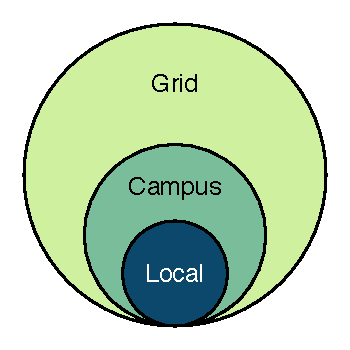
\includegraphics{images/BoscoGrowing.pdf}
	\caption{Bosco's Growing Reach as Demand Increases}
	\label{fig:boscogrowing}
\end{figure}

A framework for job submission to remote resources which the user does not control.  Typical grid submission is done to custom interfaces such as the Globus Resource Allocation Manager \cite{foster1999globus} (GRAM), which are previously installed by an administrator.  Opportunistic resources, which are abundant, typically do not have specialized grid software installed.  Further, grid submission software adds administrator overhead for maintenance.  I propose a framework that does not require administrator intervention for remote submission to opportunistic resources.  The framework uses interfaces that are installed on nearly all clusters that are typically used for interactive access.  It automates the submission and error handling of jobs submitted to remote resources, while providing the user a consistent interface over multiple, load balanced clusters.


But Bosco is not enough for researchers that have large data requirements.  Therefore, we must consider data transfers and storage on the campus.


%Most major research campuses, whether a university campus, or a national lab campus, have a research computing resource.  The computing resources are broken into two categories:

%\begin{itemize}

%\item Condominium - Resources are purchased by research groups for their dedicated use.  They are added to a cluster that may share infrastructure such as a filesystem or an interconnect.
%\item Shared resources -  Resources are purchased by a central authority that are shared between multiple research groups.

%\end{itemize}





\section{Data Transfers on Campus}

Data management and distribution has become a bottleneck in for scientific computing.  For batch computing, the impediment is transferring the data from the user's computer to the execution resources.  Large data workflows can strain the network near the user's computer which can take unreasonable amounts of time.

As users spread their computation across multiple clusters either on the campus or across campuses, data distribution and collection becomes more difficult.  Before using the campus grid, a user would select a cluster to do their processing.  The user then could host all of their data on that cluster by copying the data onto that cluster's shared filesystem.  The jobs access the data from the distributed filesystem just as it would on the user's desktop, available for all executions at the same directory.

These assumptions do not hold for a campus grid.  A grid is made up of multiple computational clusters, with potentially many separate file systems.  There is no single filesystem that a user can access from every computational resource.  Therefore, the data must be handled differently than when on a shared filesystem.  


Most distributed batch schedulers are able to transfer the input data for each job execution.  Each job starts with an empty sandbox and the scheduler will transfer the files into it.  When the user is not using the scheduler to transfer data, the input data must still reach the execution host.  Data will be transferred from the source (usually the user's computer) to the execution resources for processing.  The network connection between the source and the execution resources may be a bottleneck for the computation.  Frequent re-transfers of the same input data will further congest the network between the source and the execution resources.

In this dissertation, I optimized two attributes of distributed data management: efficient transfer methods and reduction of duplicate transfers.

I introduce the CacheD, a caching and data transfer daemon for input data in distributed computing.  The CacheD uses novel data transfer methods based on technology developed for large data transfers on the internet, BitTorrent.  It also caches input data on the execution resources to enable quick transfers on subsequent requests for the same input data.



\section{Data Distribution Policy Language}
The data must flow from the data source to the computational resource in an efficient manner.  For this reason, it is necessary to extract information about the data from the user, such as if it is shared between many jobs, or unique to each and every job.  Further, some data needs to be protected, therefore we must learn if the data is private or public.  Different transfer methods are necessary for different data types.  For example, if the data is shared between many executions, then it may be cached or can be group transferred.  

Some of these job attributes can be extracted from the job submission files without explicit instructions.  Input files that are shared between multiple executions can be categorized as shared.

A modern flexible policy language for describing data handling for computation coordination.  Users of grid submission software have to explicitly define how their files will be transferred from their submission host to the remote execution resource where the data will be consumed.  They have to coordinate with the storage resources and the computation on their own.  I propose a policy language that allows the scheduler to decide an appropriate method for data transfer.  It determines the transfer method by negotiating between the following 3 sources: a user-given policy language for the data, the remote execution resource's capabilities and preferences, and the submitting resource's capabilities and preferences.  

The user-given policy language specifies if the data is private or public, and whether the data is shared between multiple jobs or is unique to each job.  This negotiation can be used to hide data transfer details from the user while optimizing data transfers between the submission host and the execution resources.


\section{Overview of Dissertation}

This dissertation describes how data intensive applications can be rn in a distributed campus environment.   is broken down into multiple chapters.  

\begin{description}
	\item[Chapter \ref{chapter:relatedwork}:]  Distributed computing and storage has a computational 
	\item[Chapter \ref{chapter:campusjobs}:] we will discuss how computing can be managed on the campus using the Bosco manager.  This chapter expands on my masters thesis.  But Bosco is not enough for researchers with large data requirements.  Therefore, we research methods to expedite data transfer on the campus.
	\item[Chapter \ref{chapter:campusdata}:] discusses these methods for describing and moving data on the campus
	\item[Chapter \ref{chapter:coordinatingstorage}:]
\end{description}

In Chapter \ref{chapter:relatedwork}, I will discuss work related to my research.  

In Chapter \ref{chapter:campusjobs} 

Chapter \ref{chapter:campusdata} .  Chapter \ref{chapter:coordinatingstorage} describes a method for coordinating storage with computing using a policy language for data transfers and transfer decisions, and includes a novel transfer technique for large shared data on the campus.


\newpage
\section{A Note on Terms}

\begin{description}
	\item[Job:] A packaged unit of work with input and output.  A job may consuming computational, memory, and/or storage resources in a batch system.
	\item[Workflow:] A sequence of jobs executed on resources.  The jobs may have some ordering.
	\item[Campus:] An administrative domain where all resources have similar access policies.
	\item[Execution Resource:] A resource which fulfill the requirements of a job, and may run it.  This may be a worker node in a cluster.
	\item[Cluster:] A set of execution resources that have high interconnection bandwidth and are managed by a single scheduler.
\end{description}



